\documentclass[./some_latex_template.tex]{subfiles}
\begin{document}

\title{Randomized Algorithms for $\bA\bx = \bb$}
\author{Benjamin Chu}
\maketitle

\textbf{Problem statement:} Given matrix $\bA$ and vector $\bb$, find vector $\bx$ such that $\bA \bx = \bb$.

\section{Review}

\noindent Some motivating examples:

\begin{itemize}
	\item Least squares seek the solution to $\bX^t\bX \bbeta = \bX^t \by$. 
	\item PDE solvers and finite element methods
	\item Image reconstruction: a series of angular projections (i.e. sinogram) can be used to reconstruct an image. 
\end{itemize}

\noindent Notable computational challenges

\begin{itemize}
	\item $\bA$ may be large: a dense $10^6 \times 10^6$ float64 matrix is 6 terabytes
	\item $\bA$ may be fat\&short or tall\&skinny, so $\bx$ may not be unique or even exist (i.e. need approximations). 
	\item Numerical stability
\end{itemize}

\noindent Messages:
 
\begin{itemize}
	\item Never do $\bx = \bA^{-1}\bb$ for any real problem.
	\item Take advantage of $\bA$'s special structure. (e.g. sparse, sparse + rank 1 update, triangular...etc). Learn everything about numerical linear algebra in Dr. Hua Zhou's class -  biostats M280. Biomath 205 and Math 270c may be good to learn theories. 
	\item Large, dense problems requires \textit{randomized} iterative methods. 
\end{itemize}

\subsection{Direct methods for dense, small problems}

Solving $\bA \bx = \bb$ (review):

\begin{enumerate}
	\item Factorize: 
		\begin{itemize}
			\item $\bL\bU: \bA = \bL\bU, \bL =$ lower triangular matrix and $\bU =$ upper triangular
			\item $\bQ\bR: \bA = \bQ\bR, \bQ\bQ^t = \bI$ and $\bR =$ upper triangular. 
			\item Cholesky: $\bA = \bL\bL^t, \bL =$ lower triangular matrix.
		\end{itemize}
	\item Solving:
		\begin{itemize}
			\item $\bL\bU: \bA\bx = \bb \iff \bL(\bU\bx) = \bb \iff$ $\bL\by = \bb$ and $\bU\bx = \by$.
			\item $\bQ\bR: \bA\bx = \bb \iff \bQ\bR\bx = \bb \iff \bR\bx = \bQ^t\bb$
			\item Cholesky: $\bA\bx = \bb \iff \bL\bL^t\bx = \bb \iff \bL^t\bx = \by$ and $\bL\by = \bb$. 
		\end{itemize}
	\item Remarks:
		\begin{itemize}
			\item Last step in (2) uses backward substitution due to triangular structure. 
			\item For non-square matrices, step (1) uses QR (in general).
			\item For square matrices, 
				\begin{itemize}
					\item If $\bA$ is positive definite, step (1) use Cholesky (in general).
					\item Otherwise, step (1) uses LU (in general). 
				\end{itemize}
			\item Other methods (e.g. householder, modified Gram Schmidt, SVD, sweep) may be useful in certain cases. 
			\item When are QR/LU/Cholesky preferred over iterative/stochastic-iterative algorithms?
		\end{itemize}
\end{enumerate}

\begin{examplebox}{\textbf{Direct methods require "small" matrices}}{}
My 2019 macbook pro with 8 Intel Core i9-9880H CPUs have 423.2 GFLOPS computing power total. Thus, it runs 423,200,000,000 (single precision) floating point operations per second. Algorithms like QR/LU scale as $O(n^3)$. How long does it take to compute a factorization for a $10,000 \times 10,000$ matrix? Ans: $10000^3 / 423200000000 \approx 2.4$ seconds. If the matrix is 10 times bigger (homework: is it possible to make this matrix on a laptop?), it would take roughly 2362 seconds, or 39 minutes. Another 10 times bigger would take 655 hours. Obviously, factorization methods break down in this regime. 
\end{examplebox}


\subsection{Iterative methods for large, sparse problems}

Large, sparse problems are usually solved by iterative methods. An iterative algorithm means an algorithm that computes a sequence of points $x_0, x_1, ..., x_k \rightarrow x_{\rm true}$ as $k \rightarrow \infty$. This algorithm converges when $x_k \approx x_{k + 1}$, which hopefully implies $x_{k} \approx x_{\rm true}$ with some reasonably small $k$. Now, one must first define what is meant by a solution $x_{\rm true}$ since $\bA$ may be over/under-determined. The following is typically used:

\begin{definitionbox}{}{}
$\bx^*$ is the solution to $\bA \bx = \bb$ if $\bx^* = \argmin_{\bx \in \R^n} ||\bA\bx - \bb||$ with respect to some norm.
\end{definitionbox}

\noindent Why do we need iterative algorithms instead of QR/LU/Cholesky for sparse systems? Even if $\bA$ is sparse, $\bL, \bU, \bQ, \bR$ is generally not sparse (e.g. consider $\bA$ with 1's along first row and column, and along the diagonal). Banded matrices is an exception. A number of non-stochastic iterative algorithms algorithms is popular:

\begin{itemize}
	\item Conjugate gradient (sparse, symmetric, positive definite)
	\item GMRES (requires good preconditioner)
	\item (L-) BFGS (requires approximate hessian)
	\item https://juliamath.github.io/IterativeSolvers.jl/dev/
\end{itemize}

\noindent If $\bA$ is not sparse enough, then one cannot load $\bA$ into RAM and the methods above break down. For large and dense problems, recent literature focuses on \textit{randomized} algorithms. We cover 2:
\begin{itemize}
	\item Stochastic gradient descent
	\item Randomized Kaczmarz (used for overdetermined systems, wiki says sparsity is needed to be superior to conjugate gradient)
	\item Randomized Gauss-Siedel, Randomized MM algorithm? 
\end{itemize}

\section{Stochastic gradient descent for large, dense problems}

When $\bA$ is dense and large, we cannot load the matrix into memory. Therefore the idea is to approximate the gradient with a subset of $\bA$. For SGD, this subset is a single row of $\bA$, denoted by $\bA_i^t$. We first begin with intuition behind gradient descent. 

\subsection{Geometric intuition of gradient descent}

\begin{center}
	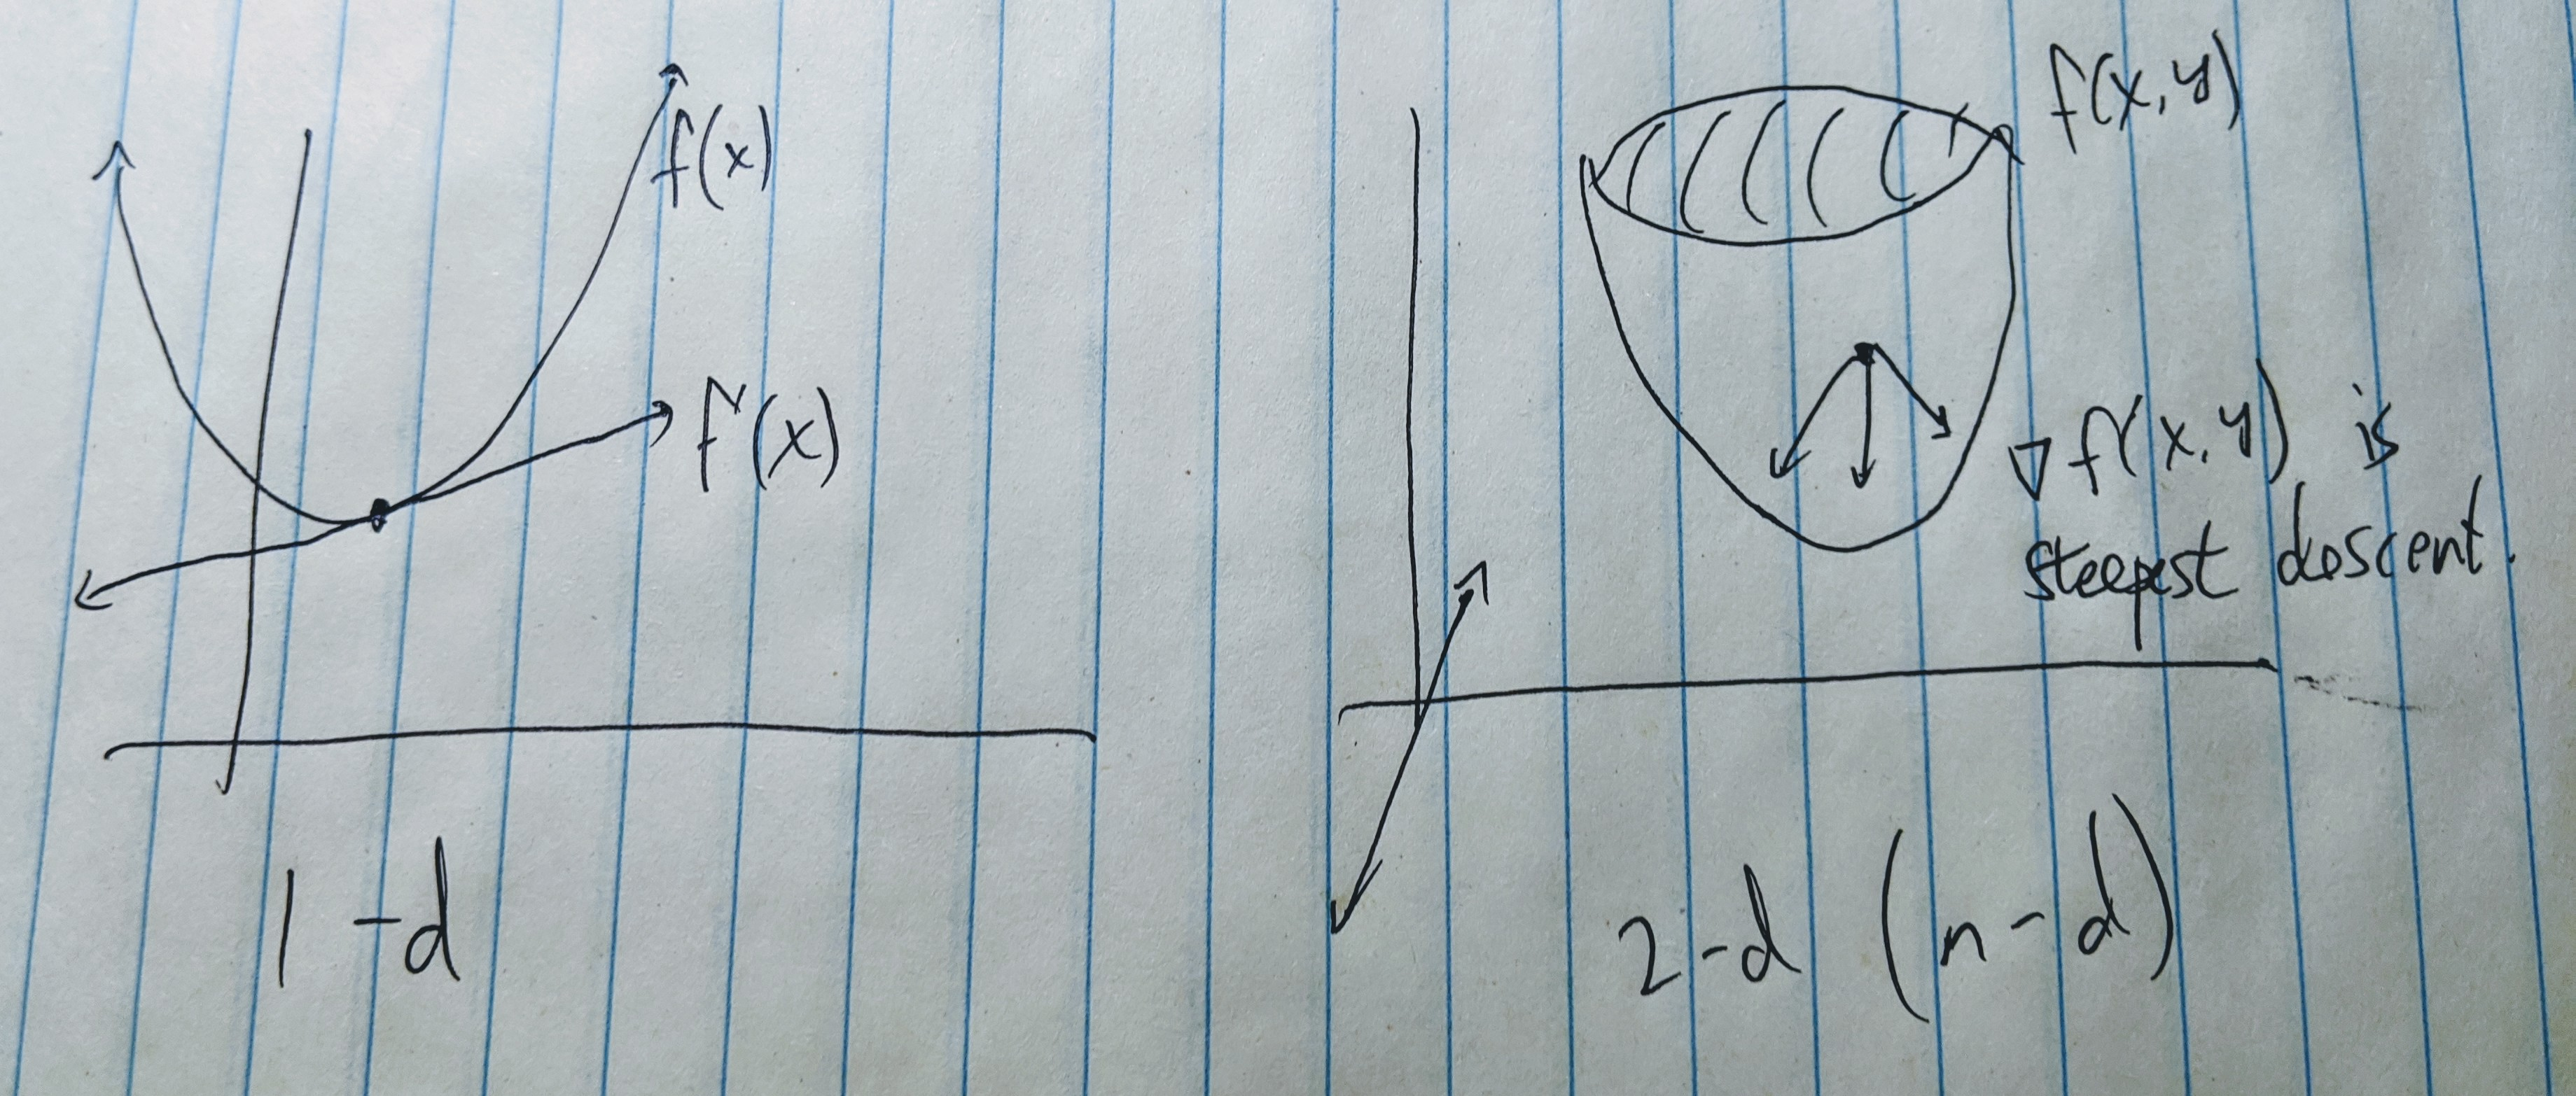
\includegraphics[scale=0.1]{gradient_illustration.jpg}
\end{center}

\subsection{Why does gradient methods work, mathematically?}

We want to solve $\bA\bx = \bb \iff \bx$ minimizes $f(\bx) = \frac{1}{2}||\bA\bx - \bb||^2_2 + \lambda||\bx||_2$. Gradient methods achieve this via iterations:
\begin{align}\label{gradient_method_works}
	\bx_{k + 1} = \bx_k - s_k \nabla f(\bx_k),
\end{align}
where $s_k$ is a positive step size. $\lambda ||\bx||_2$ term is typically added to prefer solutions with small coefficients. 

\begin{theorembox}{}{}
The iteration defined by $\bx_{k + 1} = \bx_k - s_k \nabla f(\bx_k)$ satisfies $f(x_{k + 1}) \le f(x_k)$. 
\end{theorembox}
\begin{proof}
	\begin{align*}
		f(\bx_{k + 1}) 
		&= f(\bx_k - s_k\nabla f(\bx_k)) \\
		&= f(\bx_k) - s_k\nabla f(\bx_k)^t\nabla f(\bx_k) + O(s_k^2)\\
		&= f(\bx_k) - s_k ||\nabla f(\bx_k)||_2^2 + O(s_k^2)\\
		&\le f(\bx_k).
	\end{align*}
Here the second equality is by Taylor series and the last line is because $s_k > 0$. 
\end{proof}

\begin{itemize}
	\item Geometric intuition of gradient descent. Note that $\nabla \frac{1}{2}||\bA\bx - \bb||_2^2 = \bA^t(\bA^t\bx - \bb)$ (see homework).
	\item Why does gradient methods work? (theorem showing each iteration decreases error)
	\item Explain savings in memory
	\item Idea behind SGD is how it agrees with GD \textit{in expectation}. (last part of proof requires some notation: see homework) Variance does not decrease but we don't care about that. Show example of SGD with missing data Needell's paper
	\item Convergence? Rate of convergence?
	\item Discuss parallel computing -> recall Hogwild paper claims that lockings not required if matrix is sparse (i.e. race condition is rare). 
\end{itemize}

\section{Kaczmarz and Randomized Kaczmarz method for overdetermined systems}

\begin{itemize}
	\item Krylov subspace methods
	\item Iteration scheme and geometric intuition
	\item Exponential convergence rate
	\item Does not converge to OLS solution for inconsistent systems.
	\item RK is special case of SGD with reweighted importance sampling
\end{itemize}

\section{Problems}
In honor of Ken Lange, you are required to do 2 problems. If you do more I will grade your top 2 problems. Every problem is worth the same number of points. If a problem has subproblems, each subproblem is worth the same number of points.

\begin{problembox}{{BLAS is better than you}}{}
Consider the problem of dense matrix-vector multiplication. 
\begin{enumerate}
	\item Write your own matrix-vector multiplication routine in Julia.
	\item Compare your code's speed (consider using \texttt{BenchmarkTools.jl}) to BLAS routines on $\bX \in \R^{n \times n}$ matrices where $n = 100, 1000$, and $10000$. Which is faster?
	\item \textit{Parallelize} your code using Julia's built-in multithreading (suitable for single machine parallel code) or \texttt{Distributed.jl} package (suitable for multi-core distributed computing), then perform the comparison. What is the speedup in your code? Did you have to use additional memory? How close are you to beating BLAS?
\end{enumerate}
\end{problembox}

\begin{problembox}{Sparse matrices is somtimes better than BLAS}{}
Consider the problem of dense matrix-vector and matrix-matrix multiplication when the matrices involved is potentially sparse. 
\begin{enumerate}
	\item Suppose $\bX \in \R^{n \times n}$ where $n = 10^6$. How much RAM  memory is required (in gigabytes) to store a dense matrix in double precision (i.e. Float64)? In single precision (Float32)? Half precision (Float16)? You will need at least this much RAM in order to create a matrix of this size. 
	\item If $n = 10^6$ and only $1\%$ of the entries are non-zero, how much memory do you need to store a sparse double precision matrix? Create such a matrix with Julia's \texttt{SparseArrays.jl} and verify your guess with Julia's \texttt{sizeof()} command. 
	\item Using functions associated with Julia's \texttt{SparseArrays.jl}, generate \textit{sparse} matrices with sizes $n = 10^4, 10^5, 10^6$ and with sparsity level $0.001, 0.01, 0.1$. Convert these matrices to \textit{dense} matrices (hint: is this possible?), and compare the speed of a (sparse) matrix-vector and matrix-matrix multiplication to a (dense) matrix-vector and matrix-matrix multiplication. Why is BLAS slower in some cases but not others? Use dense vectors for the matrix-vector multiplication. 
\end{enumerate}
\end{problembox}

\begin{problembox}{Exact 2nd order Taylor's expansion}{}
Suppose $f$ is continuous and twice differentiable. Show that there exists $y \in (x_0, x)$ such that:
\begin{align*}
f(x) = f(x_0) + f'(x_0)(x - x_0) + \frac{1}{2} f''(y)(x - x_0)^2.
\end{align*}
This fact is used (in chapter 9.2, without proof) to motivate the quadratic upper bound principle used ubiquitously in MM algorithms. 
\end{problembox}

\begin{problembox}{Notation problem}{}
Let $\bX \in \R^{n \times p}$, $\lambda_i \in \R$, and $\bx_i^T \in \R^{1 \times p}$ be row $i$ of $\bX$. Show that
\begin{align*}
	\sum_{i=1}^n \lambda_i \bx_i\bx_i^T = \bX^T
	\begin{bmatrix}
		\lambda_1 & & \bzero \\
		& \ddots & \\
		\bzero & & \lambda_n
	\end{bmatrix} \bX
\end{align*}
This is standard notation (e.g. used in section 3.4 of \cite{dobson2008introduction}), and in my proof that SGD agrees with GD in expectation. 
\end{problembox}

\begin{problembox}{L2 norm enjoys nice quadratic behavior}{}
Let $\bA \in \R^{n \times p}, \bx \in \R^{p}$ and $\bb \in \R^n$.
\begin{enumerate}
	\item Compute the gradient of $F(\bx) = \frac{1}{2}||\bA\bx - \bb||^2_2$.
	\item Compute the gradient of $f_i(\bx) = \frac{1}{2} (\bA_i^t \bx - \bb_i)^2$ where $\bA_i^t \in \R^{1 \times p}$ is row $i$ of $\bA$. 
\end{enumerate}
\end{problembox}

\bibliographystyle{apalike}
\bibliography{references}

\end{document}